
%%%%%%%%%%%% STRUCTURE %%%%%%%%%%%%%%%
\documentclass[a4paper,12pt]{article}
\usepackage[T1]{fontenc}
\usepackage[utf8]{inputenc}
\usepackage[brazil]{babel}
\usepackage{lmodern}
\usepackage{setspace}
\usepackage[top=2cm, bottom=2cm, left=2cm, right=2cm]{geometry}
%%%%%%%%%%%%%%%%%%%%%%%%%%%%%%%%%%%%%%

%%%%%%%%%%%%%%%% PAGES STYLE %%%%%%%%%
\usepackage{fancyhdr}
\fancypagestyle{main}{
\renewcommand{\headrulewidth}{0pt}
\fancyhead[RO]{\thepage}
\fancyfoot[CO]{}
}
%%%%%%%%%%%%%%%%%%%%%%%%%%%%%%%%%%%%%%

\usepackage{graphicx}
\usepackage{epstopdf}
\usepackage{subfig}
\usepackage{mathptmx}
\usepackage{amsmath}
\usepackage{changepage}
\usepackage{cite}
%\usepackage[alf]{abntex2cite}

%%%%%%%%%%% PDF METADATA %%%%%%%%%%%%%
\usepackage[ pdftitle={MODELO RELATÓRIO},
pdfsubject={INTRODUÇÃO AO LABORATÓRIO DE CONTROLE - Grupo 3},
pdfkeywords={Controle,Automação,UFRN,DCA,ipump},
hidelinks]{hyperref}
%%%%%%%%%%%%%%%%%%%%%%%%%%%%%%%%%%%%%%

\begin{document}

\onehalfspacing

\thispagestyle{empty}

\setcounter{page}{1}

%%%%%%%%%%%% LOGOS %%%%%%%%%%%%%%%%%%%

\begin{figure}[!ht]

\centering

\subfloat{

\includegraphics[width=2.7cm]{UFRN.eps}
\label{UFRN Logo}
}
\hspace{11.09cm}
\subfloat{

\includegraphics[width=2.4cm]{DCA.eps}
\label{DCA Logo}
}

%\caption{}
\label{Logos}

\end{figure}

%%%%%%%%%%%%%%% CAPA %%%%%%%%%%%%%%%%%

\vspace{-1cm}

\begin{center}
{\bf{\normalsize UNIVERSIDADE FEDERAL DO RIO GRANDE DO NORTE\\
CENTRO DE TECNOLOGIA\\
DEPARTAMENTO DE ENGENHARIA DE COMPUTAÇÃO E AUTOMAÇÃO\\
CURSO DE ENGENHARIA MECATRÔNICA
}}


\vspace{3.6cm}

{\bf{\large RECAM: MÓDULO DE GRAVAÇÃO INTELIGENTE PARA CÂMERAS DE SEGURANÇA, BASEADO NA DETECÇÃO DE FACES EM CENA.
}}
\vspace{0.4 cm}
{\large \\}

\vspace{5.6cm}



\begin{flushright}
\begin{normalsize}

JOELSON DE CARVALHO ROCHA JÚNIOR: 20160153946\\
\vspace{0.8cm}

\end{normalsize}
\end{flushright}


\vspace{6 cm}

{\large Natal-RN\\
2017}

\end{center}

\newpage

%%%%%%%%%%%%%%%  CONTRA-CAPA %%%%%%%%%

\thispagestyle{empty}

\begin{center}
\begin{normalsize}

JOELSON DE CARVALHO ROCHA JÚNIOR: 20160153946\\
\vspace{0.8cm}
 

\end{normalsize}
\end{center}
\vspace{3cm}

{\bf{\large \centering RECAM: MÓDULO DE GRAVAÇÃO INTELIGENTE PARA CÂMERAS DE SEGURANÇA, BASEADO NA DETECÇÃO DE FACES EM CENA.
	}}

\vspace{4cm}

\begin{adjustwidth}{7.5cm}{0cm}

{\normalsize

Relatório apresentado à disciplina de
Processamento Digital de Imagens - DCA0445, correspondente à
avaliação da 3ª unidade do semestre 2017.2 do curso de Engenharia de Computação e Automação da
Universidade Federal do Rio Grande do Norte, sob
orientação do {\bf Prof. Dr. Agostinho de Medeiros Brito Júnior}
}

\end{adjustwidth}

\vspace{2cm}

\begin{center}

Professor:  \center{Agostinho de Medeiros Brito Júnior}\\ 

\vspace{5.0cm}

{\large Natal-RN\\
2017}

\end{center}

\newpage

%%%%%%%%%%%%%%%  RESUMO %%%%%%%%%%%%%%

\thispagestyle{empty}

\begin{center}
{\large \textbf{RESUMO}}
\end{center}

\vspace{3cm}

\begin{flushleft}

\hspace{4ex}O presente relatório busca demonstrar o desenvolvimento, em software, de um módulo para câmeras de segurança com o objetivo de realizar a gravação de vídeo baseando-se no algorítmo de detecção de faces de Viola-Jones, permitindo assim o uso de dispositivos de alta resolução em sistemas de vigilância. Ao final de seu desenvolvimento, foram obtidos resultados satisfatórios tais como: redução no tamanho do arquivo de gravação gerado, devido a redução do tempo do vídeo final.\\

\end{flushleft}

\vspace{1.5cm}

\textbf{Palavras-chave: Gravação de vídeo. Câmeras de segurança. Detecção de faces. Viola-Jones. Resolução.}

\newpage

%%%%%%%%%%%%%%%  LISTA DE SÍMBOLOS %%%



%%%%%%%%% LISTA DE FIGURAS %%%%%%%%%%%

\thispagestyle{empty}

\begin{center}
\listoffigures
\end{center}

\newpage

%%%%%%%%%%%%%%% SUMÁRIO %%%%%%%%%%%%%%

\thispagestyle{empty}

\begin{center}
\tableofcontents
\end{center}

\newpage

%%%%%%%%%%%%%%% INTRODUÇÃO %%%%%%%%%%%

\thispagestyle{main}

\section{INTRODUÇÃO}

\begin{flushleft}
	
\hspace{4ex}Sistemas de monitoramento remoto se tornaram cada vez mais comuns em estabelecimentos de toda natureza (comerciais, públicos, residenciais etc.). Existem vários motivos para o uso dessa tecnologia, desde a inibição de tentativas de assalto até ao estudo comportamentamental de indivíduos (animais ou humanos).


\hspace{4ex}Infelizmente, em noticiários de todo o mundo, há vários registros de cenas onde a presença de câmeras não tem surtido efeito na ação criminosa de bandidos, conforme Fabrício\cite{fab}. Em muitos casos não há como identificar quais pessoas participaram do ocorrido, devido a limitação encontrada na transmissão de dados da rede utilizada. Por exemplo: para que sejam reproduzidos, simultaneamente e com alta qualidade, vídeos de 6 câmeras de vigilância em uma farmácia, se faz necessário investir em um computador com alta capacidade de processamento e em uma rede com alta taxa de transferência de dados. A solução encontrada por muitas pessoas é diminuir a resolução das câmeras, produzindo imagens como a da Figura \ref{lowresolutioncamera}. 
\begin{figure}[h!]
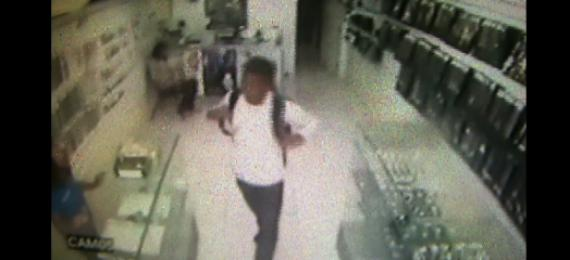
\includegraphics[scale=.85]{01-circuitointerno.jpg}
\caption{Câmera de circuito interno em baixa resolução.}
\label{lowresolutioncamera}
\end{figure}

\hspace{4ex} Nota-se que essa abordagem permite ao usuário ter um registro do que ocorreu a cena, porém, na grande maioria dos casos a identificação do(s) indivíduo(s) em cena se torna impossível.

\end{flushleft}
\subsection{Proposta do projeto}
\hspace{4ex}Este projeto propõe a elaboração de um módulo para câmeras de segurança que otimize a reprodução, simultânea, de vídeos em alta resolução, permitindo com que o usuário possa identificar, de forma mais rápida, pessoas em cena.

\newpage

%%%%%%%%%% REFERENCIAL TEÓRICO %%%%%%%

\thispagestyle{main}

\section{REFERENCIAL TEÓRICO}
\subsection{Reconhecimento de objetos com Viola-Jones}
\hspace{4ex}Em 2001, Paul Viola e Michael Jones\cite{vj} propuseram uma técnica de detecção de objetos chamada "Rapid Object using a Boosted Cascade of Simple Features", que apresenta  uma sugestão voltada a detecção de faces frontais utilizando técnicas que prometem processamento de imagens extremamente rápidos e o alcance de altas taxas de detecção. A técnica foi dividida em 3 partes: 
\begin{itemize}
	\item {\bf Imagem Integral}: conceito que permite que o detector compute caraterística de forma mais rápida;
	\item {\bf Aprendizado baseado em AdaBoost}: seleciona características mais importantes de um grande conjunto de classificadores;
	\item {\bf Classificadores em cascata}: aplicam classificadores mais complexos à medida que a imagem analisada passa por estágios classificatórios.
\end{itemize}
\subsubsection{Imagem Integral}
\hspace{4ex} Esse procedimento classifica imagens baseando-se em 3 características simples denominadas de "características retangulares", sendo elas de dois, três e quatro retângulos. Elas nada são filtros aplicados à regiões da imagem, conforme ilustradas na Figura \ref{imagemintegral}.

\begin{figure}[h!]
	\centering
	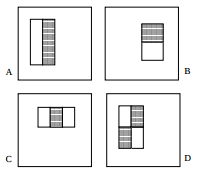
\includegraphics[scale=1]{imagemintegral.png}
	\caption{Característica de dois retângulos é mostrada em [A] e [B], de três em [C] e de quatro em [D].}
	\label{imagemintegral}
\end{figure}
 
\hspace{4ex}O procedimento para cálculo da imagem integral é feito da seguinte forma: O valor de cada pixel da matriz da imagem integral é equivalente a soma dos valores de todos os pixels da matriz que estão imediatamente acima e à esquerda desse pixel, incluindo seu próprio valor, conforme a Equação \ref{eq:imgintegral}.
\begin{equation} \label{eq:imgintegral}
	ii(x,y)=\sum_{x'\le x,y'\le y}^{} i(x',y')
\end{equation}

\hspace{4ex}De forma mais eficiente, é calculado o valor da imagem integral utilizando os valores já adquiridos da imagem. Dessa forma o método não realiza várias adições. A expressão 2 explicita tal raciocínio, onde $i(x,y)$ representa o pixel da imagem e $ii(x,y)$, o da imagem integral.
\begin{equation}\label{eq:imgintotm}
	ii(x,y)=i(x,y)+ii(x-1,y)+ii(x,y-1)-ii(x-1,y-1)	
\end{equation}


\thispagestyle{main}
\subsubsection{Aprendizado baseado em AdaBoost}

\hspace{4ex}É utilizado para selecionar pequenos conjuntos de características e treinar os classificadores utilizados para detecção de objetos, aumentando assim a performance de classificação de algorítmos simples de aprendizagem.

\hspace{4ex}De acordo com Rojas(2009)[x], esse algorítmo foi proposto por Yoav Freund e Robert Shapire, em 1995, como um método que é capaz de gerar um forte classificador à partir de um conjunto fraco. O método testa, classifica e atribui pesos à cada classificador, que por sua vez, são combinados, juntamente com seus pesos, e compõem um classificador mais robusto e eficiente.

\hspace{4ex}Os pesos são ajustados a cada iteração, bem como os classificadores, retreinados utilizando uma determinda característica. Feito isso, o erro é calculado para cada classificador, escolhe-se o que possuir menor magnitude de erro e então os pesos são reajustados para se dar início a uma nova iteração. Por fim, o classificador mais forte é escolhido à partir de classificadores mais fracos, e é dados pela combinação linear entre eles e seus respectivos pesos como ilustrado na Equação \ref{adaboost}.

\begin{equation}\label{adaboost}
	C_{(m)}=\alpha_{1}k_{1}(x_{i}) +\alpha_{2}k_{2}(x_{i})+...+\alpha_{m}k_{m}(x_{i})
\end{equation}

\hspace{4ex}Onde: $C_{(m)}$ é o conjunto de classificadores, $m$ o número de iterações,$\alpha$ o peso relacionado a cada classificador, $k$ o classificador e $x$ o padrão. 

\hspace{4ex}Após utilizar o método, selecionando uma característica dentre as 180.000 possíveis, Viola e Jones relatam em seu trabalho que as duas características retangulares mais fortes acontecem geralmente em duas regiões próximas aos olhos:
\begin{itemize}
	\item região dos olhos em constraste com as do nariz e bochechas;
	\item região dos olhos em constraste com a do osso do nariz.
\end{itemize}

\hspace{4ex}É possível observar o resultado na Figura \ref{adboost}.

\begin{figure}[h!]
	\centering
	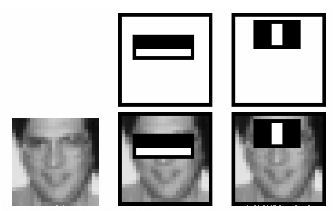
\includegraphics[scale=.5]{adaboost.png}
	\caption{Melhores características selecionadas pelo algorítmo de AdaBoost.}
	\label{adboost}
\end{figure}



\subsubsection{Classificadores em cascata}
\hspace{4ex}São utilizados para reduzir a imagem em regiões que contenham o objeto de interesse, aumentando assim a performance do método.

\hspace{4ex}Classificadores mais simples são aplicados à regiões da imagem.Caso a região passe na avaliação, ela é submetida a classificadores mais complexos, caso contrário, ela é descartada. Essa estratégia reduz o número de subjanelas a serem analizadas, e consequentemente o número de ocorrências de falsos positivos.

\hspace{4ex}O treinamento do classificador se dá na forma de troca equivalente, ou seja, os classificadores que possuem mais características possuem maior taxa de detecção.
\thispagestyle{main}
\section{METODOLOGIA}
\hspace{4ex}O projeto foi desenvolvido na linguagem Python. Utilizou-se a biblioteca de processamento de imagens OpenCV3.0\cite{opencv} , WebCam USB bem como o sistema para controle de versões GIT. Também foi utilizado o treinador para detecção de faces frontais, disponibilizado pelo openCV. Foram feitas consultas no livro do Gonzalez\cite{PDI} durante a disciplina que auxiliam no entendimento do algorítmo.

\hspace{4ex}O código desenvolvido entitulado de $main.py$ segue abaixo na Figura \ref{script}.

\begin{figure}[h!]
	\centering
	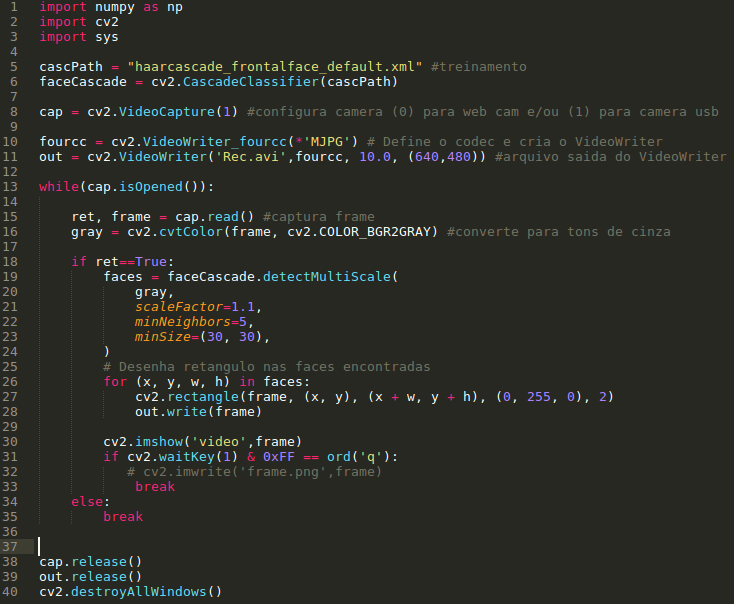
\includegraphics[scale=.5]{script.png}
	\caption{Código comentado para uso no módulo ReCam.}
	\label{script}
\end{figure}

\newpage
\thispagestyle{main}
\section{RESULTADOS}
\hspace{4ex}O resultado obtido após meia hora de funcionamento do módulo foi um vídeo de 21 segundos onde só aparecem as pessoas em cena, conforme a figura \ref{resultado}.

\begin{figure}[h!]
	\centering
	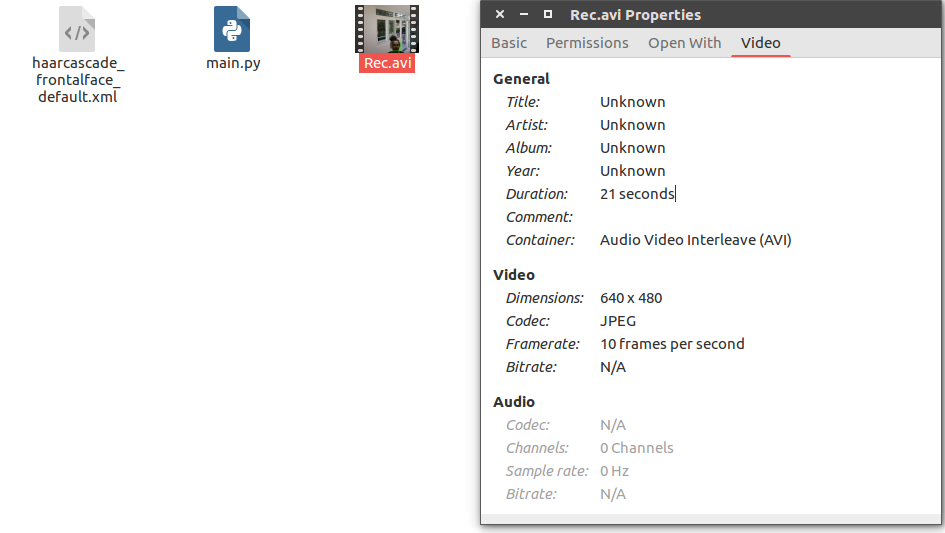
\includegraphics[scale=.5]{resultado.png}
	\caption{Imagem resultante.}
	\label{resultado}
\end{figure}

\hspace{4ex} Em suma, foi possível observar que realmente este tipo de abordagem é promissora. Provavéis melhorias serão implementadas para aprimorá-lo, tais como: utilizar o ReCam em um Raspberry Pi e conseguir utilizá-lo com o auxílio do sistema supervisório ZoneMinder.


\newpage
%%%%%%%% REFERÊNCIAS %%%%%%%%%%%%%%%%%



\thispagestyle{main}
% Referências bibliogáficas (geradas automaticamente)
\addcontentsline{toc}{chapter}{Referências Bibliográficas}
\bibliographystyle{ieeetr}
\bibliography{bib/bibliografia}




\end{document}